\documentclass[pdflatex,sn-nature]{sn-jnl}


\usepackage{graphicx}%
\usepackage{multirow}%
\usepackage{amsmath,amssymb,amsfonts}%
\usepackage{amsthm}%
\usepackage{mathrsfs}%
\usepackage[title]{appendix}%
\usepackage{xcolor}%
\usepackage{textcomp}%
\usepackage{manyfoot}%
\usepackage{booktabs}%
\usepackage{algorithm}%
\usepackage{algorithmicx}%
\usepackage{tabularx}
\usepackage{algpseudocode}%
\usepackage{listings}%
\usepackage{csquotes}
\usepackage{placeins}
%\usepackage{float} % sn-nature class might include this or similar functionality

\theoremstyle{thmstyleone}%
\newtheorem{theorem}{Theorem}
\newtheorem{proposition}[theorem]{Proposition}
\theoremstyle{thmstyletwo}%
\newtheorem{example}{Example}%
\newtheorem{remark}{Remark}%
\theoremstyle{thmstylethree}%
\newtheorem{definition}{Definition}%
\raggedbottom
\begin{document}

\title[Article Title]{Predictive Analysis of Autism Spectrum Disorder (ASD) Traits: Integrating Supervised Machine Learning and Exploratory Data Insights}


\author[1]{\fnm{Subhra} \sur{Kolay}}\email{subhrokolay2@gmail.com}

\author[2]{\fnm{Srijan} \sur{Samaddar}}\email{srijansamaddar04@gmail.com}
\equalcont{These authors contributed equally to this work.}

\author[1]{\fnm{Ayushman} \sur{Bhattacharya}}\email{bhattacharyaa599@gmail.com}
\equalcont{These authors contributed equally to this work.}

\author*[1]{\fnm{Bidisha} \sur{Bhabani}}\email{bidisha035810@gmail.com}
\equalcont{These authors contributed equally to this work.}

\affil*[1]{\orgdiv{CSE}, \orgname{JIS University}, \orgaddress{\street{ Nilgunj Rd}, \city{Kolkata}, \postcode{700109}, \state{West Bengal}, \country{India}}}

\affil[2]{\orgdiv{IT}, \orgname{NSCE}, \orgaddress{\city{Kolkata}, \postcode{700152}, \state{West Bengal}, \country{India}}}

\maketitle
\begin{center}
\textbf{Abstract}
\end{center}
\abstract*{ This research investigates the application of Supervised Learning (SL) strategies inside the machine learning (ML) space for the forecast of Autism Spectrum Disorder (ASD), a neuro-developmental condition with long lasting impacts on communication, cognition, and social abilities. We explored Logistic Regression, Decision Trees, K Closest Neighbors (KNN), Naive Bayes, Random Forest, Support Vector Machine (SVM), and Hoistogram Gradient Boosting (HGBC) techniuqes. Imperatively, we found that the Histogram Angle Boosting Classifier (HGBC) accomplished the most elevated precision (97.86 \%) in foreseeing ASD characteristics. This result, coupled with investigation of accuracy, precison, recall \& F1-score, highlights the potential of HGBC as an important technique for early ASD detection and warrants advance examination. The research is important to healthcare, advertising a promising road for moving forward towards ASD screening procedures. Particularly, when we indulge into the distribution of the AGE vs. ASD, the analogy makes it clear that the diseases affects 60 \% of the children making it prone to the younger age and the newbies, happening more commonly in males than females.} \\
\textbf{\textbf{Keywords:}}
\keywords*{Autism Spectrum Disorder (ASD), Supervised machine learning, Classification Algorithms, Logistic
Regression, KNN, SVM}.



\section{Introduction}\label{sec1}

Autism Spectrum Disorder (ASD) is a complex neuro-developmental condition characterized by symptoms such as social anxiety, lack of proper social interaction, less talk, difficulty in expressing. It has been estimated that around 1 in 31 (3.2\%) children aged 8 years have been identified with ASD\cite{1in31}, making early diagnosis and intervention crucial for improving outcomes. Early detection of ASD can significantly develop the lives of individuals.

Traditional method to diagnosing ASD generally rely on observation, behavioral assessments\cite{ini3}. However this methods are inconsistent, time-consuming and is prone to human error. Use of machine learning algorithms offer the potency to analyze large dataset on ASD and identify patterns that are more consistent and effective.

 This study aims to explore the use of various supervised machine learning algorithms for the predictive analysis of ASD triads based on the datasets available on Kaggle. The data set contains A0, A1, A2, ... upto A10 fields. These are basically boolean fields having either \enquote{YES} or \enquote{NO} to the symptoms of ASD. Aside of this, there are many criteria such as age, sex, ethnicity, family history of ASD, and results from the Autism Spectrum Quotient (AQ) test that can be considered. By applying machine learning models to this data we tried to find the best possible patterns that are most responsible for ASD. These patterns can provide valuable insight on the factors that contribute to the disorder\cite{bib12}.

 In this research, the prediction of ASD traits is carried out using various supervised machine learning models. Data pre-processing, including steps such as normalization, train-test splitting, and label encoding, was used to prepare the dataset for the model training. Various classification algorithms Logistic Regression, Decision Tree, KNN, Naïve Bayes, Random Forest, SVM, and Histogram Gradient Boosting Classifier (HGBC) were utilized to evaluate the performance metrics such as confusion matrix, precision score, F1 score, recall, and accuracy\cite{bib14}. HGBC was found to deliver the highest accuracy among all the supervised classification model. The dataset is chosen from the Kaggle and subjected to exploratory data analysis to find the relationships among features which are in the dataset such as age, sex, ethnicity, and Autism Quotient scores. Also, Hyperparameter tuning was performed to enhance model performance, improving the solidity of ASD detection.

The research contribution to the study of ASD are thus being outlined below:

\begin{itemize}
    \item \textbf{Data Modality:} Unlike this work was supervised using demographic and questionnaire-based data (eg,. AQ score, age, sex), where this Schielen et al. (2024), was conducted by neuroimaging data such as rsfMRI, sMRI, and dMRI. A lowcost option to neuroimaging MRI-based diagnostics has been proposed, it can be placed without specilized imaging substructure.
    \item \textbf{Comprehensive Comparative Analysis:} We conduct a thorough comparative analysis of seven different supervised machine learning algorithms (Logistic Regression, Decision Trees, KNN, Naive Bayes, Random Forest, SVM, and HGBC) for the predictive analysis of ASD traits on a publicly available dataset.
    \item \textbf{Identification of Superior Model:} Our study empirically identifies the HGBC as the most effective model among those evaluated for this specific ASD dataset, achieving high accuracy, precision, recall \& F1-score.
    \item \textbf{Model Optimization:} We demonstrate the application of hyperparameter tuning to optimize the performance of the HGBC model, showcasing how fine-tuning specific parameters can enhance predictive accuracy.
    \item \textbf{Dataset-Specific Insights:} Through detailed Exploratory Data Analysis (EDA), we provide specific insights into the demographic distribution of ASD traits within the dataset, highlighting age-related susceptibility (particularly in children), gender differences, and patterns related to ethnicity and family history.
    \item \textbf{Advocacy for Advanced ML in Screening:} By showcasing the superior performance of HGBC, the research advocates for the potential integration of advanced ensemble machine learning techniques into clinical workflows for early ASD detection and screening, offering a promising path towards more efficient and accurate diagnostic support.
\end{itemize}

The rest of the paper is structured into several sections paving our approach to predict ASD traits. \hyperref[sec2]{Related Works} reviews existing literature on applying machine learning and neuro-imaging techniques to ASD diagnosis, positioning our research within the broader field. The \hyperref[sec3]{Methodology} section details the practical steps undertaken, including the selection and pre-processing of the dataset and the description of the various supervised machine learning models employed for classification. Following this, the \hyperref[sec4]{Performance Analysis} presents the statistical analysis of the research, discussing hyperparameter tuning, defining the evaluation metrics used, and analyzing the performance of each model, including key findings from the confusion matrices, accuracy, precision, recall, and F1-scores. Following the same we explore the performance metrics in a graphical and tabular fashion in the \hyperref[sec:results]{Result Analysis} subsection, which delves into the deeper understanding of our findings in numeric terms. The paper produces an \hyperref[sec:data_analysis]{Exploratory Data Analysis} section which compares traits like Ethnicity, Sex and more addressing the probability of ASD detection correspondingly. Finally, the \hyperref{sec:conclusion}{Conclusion} summarizes the main findings, highlights the most successful model, discusses the implications of the results for early ASD detection, and suggests avenues for future research.


\section{Related Works}\label{sec2}

Authors in \cite{parlett2023applications} investigated the perceptions and attitudes of the parents regarding early predictive testing for ASD in infants. This paper helps to understand the Socio-cultural and Emotional challenges related with early diagnosis and testing, emphasizing the ethical implications and potential parental stress. Many parents do early testing due to the benefits of early intervention, concerns remain about stigma, privacy, and emotional burden. This paper shows how machine learning-based ASD diagnostic tools might be received by the public and healthcare providers.

Authors in \cite{nogay2020machine} explored how advanced machine learning models can be used in neuro-imaging data (MRI and fMRI) for diagnosing ASD. Authors emphasized how non-invasive imaging methods can be used to identify neurological biomarkers and integrate them with CNN and SVM supervised learning models. Their research offers important insights into combining ML algorithms with imaging data, improving the neuro level diagnosis accuracy for ASD.

\begin{table}[ht]
\centering
\caption{Summary of Related Works in ASD Diagnosis Using machine learning}
\label{tab:relatedworks}
\begin{tabularx}{\textwidth}{|p{3.2cm}|X|p{2.8cm}|} % Adjusted first column width slightly
\hline
\textbf{Study} & \textbf{Key Contribution} & \textbf{Technique Used} \\
\hline
Parlett et al. (2023) \cite{parlett2023applications} & Explored parental perspectives on early ASD testing and ethical implications & Socio-cultural analysis, ethical concerns \\
\hline
Nogay et al. (2020) \cite{nogay2020machine} & Applied ML to MRI/fMRI data to improve ASD diagnosis accuracy & CNN, SVM, neuroimaging \\
\hline
Parlett-Pelleriti et al. (2023) \cite{parlett2023applications} & Used unsupervised learning to detect ASD subtypes and hidden patterns & Clustering, dimensionality reduction \\
\hline
Vakadkar et al. (2021) \cite{bib4} & Compared supervised ML models for behavioral ASD diagnosis & Random Forest, SVM, Logistic Regression \\
\hline
Alves et al. (2023) \cite{bib5} & fMRI data analyzed to detect stable brain network clusters in ASD & Functional imaging, clustering \\
\hline
Mellema et al. (2022) \cite{bib6} & Benchmarked 12 ML models on fMRI/sMRI data, favoring deep learning & Deep learning, model comparison \\
\hline
Zhou et al. (2024) \cite{bib7} & Introduced GAN + Deep Q-Learning framework for diagnosis enhancement & Data augmentation, generative models \\
\hline
Rajagopalan et al. (2024) \cite{bib8} & Large-scale ML analysis of 30,000 participants using 28 features & Supervised ML, developmental traits \\
\hline
Jaradat et al. (2025) \cite{bib10} & Used eye-tracking data with hybrid models to achieve high accuracy & Non-invasive diagnosis, hybrid ML \\
\hline
Stevens et al. (2019) \cite{bib12} & Identified 16 behavioral ASD subgroups using clustering methods & Gaussian Mixture Models, hierarchical clustering \\
\hline
Eslami et al. (2021) \cite{bib13} & Developed interpretable ML for clinical fMRI-based ASD diagnosis & Interpretable ML, scalability \\
\hline
Prasad et al. (2023) \cite{bib14} & Combined deep learning and novel optimization for ASD detection & Brain MRI, hybrid deep learning \\
\hline
\end{tabularx}
\end{table}
This paper shows how unsupervised learning methods like dimensionality reduction and clustering are used in ASD research.Rather than depended on labeled data using of unsupervised techniques helped to find many hidden patterns, ASD subgroups, and possible biomarkers. The study describes the ways in which clustering algorithms have uncovered comorbidities and symptom clusters that could have gone unnoticed otherwise. Employing unsupervised learning and clinical analysis can be used to find new insights into the heterogeneity of ASD and help with individualized treatment planning is supported by this work \cite{parlett2023applications}.

This research shows the Techniques such as Logistic Regression, Decision Trees, Random Forest, and Naïve Bayes were applied to behavioral and clinical datasets. Various supervised machine learning algorithms to classify and detect ASD traits in children. Among all these techniques, authors found that Random Forest and SVM models to be the most accurate one. This study aligns with our goal of improving early detection using accessible data and adds further weight to the relevance of ML for ASD diagnosis \cite{bib4}.

This study uses functional MRI data from 500 subjects and analysis of stable Clusters to identify brain network patterns.The primary goal is to achieve high accuracy in differentiating between persons with ASD and control subjects. The paper uses functional Magnetic Resonance Imaging (fMRI) data in combination with advanced machine learning techniques to improve the accuracy of ASD \cite{bib5}.

In this paper \cite{bib6}, 12 machine learning models were optimized and compared using combinations of fMRI and sMRI features. The highest diagnostic accuracy is given by deep learning models and generalized well across different MRI datasets.

In advancing ASD identification with neuro-imaging research uses a framework combining Generative Adversarial Networks (GANs) and Deep Q-Learning that is  GARL to enhance ASD diagnosis using neuro-imaging data. The approach addresses data scarcity by augmenting datasets, improving diagnostic precision \cite{bib7}.

This paper used machine learning algorithms over 30,000 participants with high accuracy, sensitivity, and specificity based on 28 features including many developmental goals and eating pattern \cite{bib8}.

Eye-Tracking data sets are used to predict and diagnose ASD in \cite{bib10}. By using hybrid machine learning models they have achieving accuracy rates up to 98\%  highlighting the potential of non-invasive diagnostic tools.

This paper \cite{bib12} used 2,400 children with ASD sample, employs Gaussian Mixture Models and Hierarchical Clustering in that sample to identify 16 behavioral subgroups, aiding in tailored treatment approaches.

In this paper \cite{bib13} researchers have developed a  scalable and interpretable machine learning algorithms for ASD detection using fMRI data emphasizing the clinical applications.

Authors in \cite{bib14} introduced a deep learning approach combining brain MRI imaging with a novel hybrid training optimization technique to enhance ASD detection accuracy.

In summary, we can thus say that the recent researches on ASD diagnosis have seen a strong shift toward machine learning and neuro-imaging techniques. Studies have addressed the emotional and ethical complexities of early diagnosis \cite{parlett2023applications}, and there's been significant progress in applying advanced ML models—both supervised and unsupervised—to behavioral, clinical, and neuroimaging data. Techniques like CNNs, SVMs, clustering, and dimensionality reduction have helped identify hidden patterns, subgroups, and potential biomarkers \cite{nogay2020machine, parlett2023applications, bib5}. Meanwhile, deep learning and hybrid models continue to raise the bar for diagnostic accuracy across large datasets \cite{bib6, bib7, bib8}, and non-invasive tools like eye-tracking have shown promising results \cite{bib10}. Overall, the body of work suggests that AI and ML are not just enhancing ASD detection, but also enabling more personalized and scalable clinical insights \cite{bib12, bib13, bib14}. A brief of the existing works are encaged in \hyperref[tab:relatedworks]{Table \ref{tab:relatedworks}}.


\section{Methodology}\label{sec3}

This section has been divided into a few explanatory sub-sections, aimed towards explaining the process and the approach towards the prediction of ASD using the machine learning algorithms. The road-map includes finding a learning-model apt to serve the purpose, with our cleaned dataset. Following which feature-selection, implementation and performance evaluation were applied consecutively.

\subsection{Dataset Analysis}

The data set used here is based on the quantitative checklist for autism. There are around 10 questions has been used. The answers are converted into binary numbers on the basis of the answer \enquote{YES} or \enquote{NO}. It is observed that if at least five columns give \enquote{YES} then there is high probability of ASD traits, if less than 5 columns give \enquote{YES} then there are fewer ASD cases are present.

\subsection{Selection of Dataset}

There are various datasets available in Kaggle among which the best fit and accurate data set has been chosen from Kaggle. The dataset consists of 3,743 instances and 17 features, including both categorical and numerical variables. The data set contains autism spectrum condition (AQ) which measures several ASD traits such as age, sex, ethnicity, family history of ASD.

The variables are binary in form, which indicate the presence or absence of the ASD traits by labeling 1 for its presence and 0 for its absence.

\textbf{Target Variable:} The target variable in this dataset is binary, indicating the presence or absence of ASD traits. The target is labeled as 1 for individuals with ASD traits and 0 for those without.

\textbf{Input Features:} The features used for prediction include:
\begin{itemize}
    \item A1, A2, ..., A10: Autism Spectrum Quotient (AQ) scores that provide insights into ASD-related behaviors.
    \item Age, Year, Sex: Demographic information about the individuals.
    \item Ethnicity, Jaundice, Family member with ASD: Additional factors that might influence the presence of ASD traits.
    \item Individuals who completed the test: A categorical variable indicating whether the test was completed.
\end{itemize}

\subsection{Data Pre-processing}

Data preprocessing \cite{datapre} is one of the most essential steps to ensure that the machine learning models employed perform optimally. The following pre-processing techniques were applied to the dataset:

\begin{itemize}
    \item \textbf{Initial approach:} The dataset that is used has been compiled by Afarin Bargrizan and it contains categorical (as such nominal and ordinal) and binary attributes. The dataset has 3743 rows along with 17 columns. Since the data set is raw, it contains some categorical attributes, so to clean the data set, it is needed to pre-process the data set. All the nominal and ordinal attributes are converted into numerical attribute. Label Encoder is used to convert the data. Scikit learn library is used for necessary imports as such machine learning model, evaluation metrics, pre-processors.
    \item \textbf{Handling Missing Data:} The dataset contains no missing values, so there is no necessary imputation.
    \item \textbf{Categorical Variables Encoding:} Categorical variables (e.g: sex, ethnicity, jaundice status) were encoded using \textit{Label Encoding} to convert them into numerical values. This encoding allows categorical variables to be used by machine learning algorithms.
    \item \textbf{Feature Scaling:} Some algorithms, such as KNN and SVM, are sensitive to feature scaling. Therefore, all numerical characteristics were normalized using \textit{Min-Max Scaling}, which fits the features to a range between 0 and 1.
    \item \textbf{Data Split:} The dataset was split into training and testing sets using an 80:20 ratio. This means that 80\% of the data was used to train the models, and 20\% was reserved for testing and evaluating the model performance.
\end{itemize}


\subsection{Machine Learning Models}\label{sec3.4}

Several machine learning algorithms were employed to predict the presence of ASD traits. These models were chosen due to their popularity in classification tasks and their ability to handle various types of data. Since our dataset is non-linear and the target variable is binary, we used classification machine learning models.

The models used in this study are listed below:

\begin{itemize}
    \item Logistic Regression
    \item Decision Trees
    \item KNN
    \item Naïve Bayes
    \item Random Forest
    \item SVM
    \item HGBC
\end{itemize}
    


\section{Performance Analysis}\label{sec4}

In this research, 7 different machine learning classification models have been employed to predict ASD traits. These included Logistic Regression, Naive Bayes (different variants such as Gaussian, Bernoulli, and Multinomial were considered, though not all might be explicitly reported depending on performance), SVM (using Polynomial and Radial Basis Function kernels to handle potential non-linearity and dataset imbalance), KNN (using Euclidean and Manhattan distances), Random Forest, Decision Tree, and HGBC. Hyperparameter tuning was performed for the HGBC model to optimize performance, as it demonstrated promising initial results.

\subsection{Hyperparameter Tuning}\label{sec:hptuning}

Hyperparameter tuning was applied to the HGBC \cite{hist} to find the optimal set of parameters for maximizing performance on our dataset. The package \texttt{gradientsearchCV} is used for this process. The key parameters \cite{para} explored includes \texttt{n\_estimators}, \texttt{learning\_rate}, \texttt{max\_iter}, \texttt{max\_depth}, \texttt{min\_samples\_leaf}, and \texttt{l2\_regularization}.

\begin{figure}[ht]
    \centering
    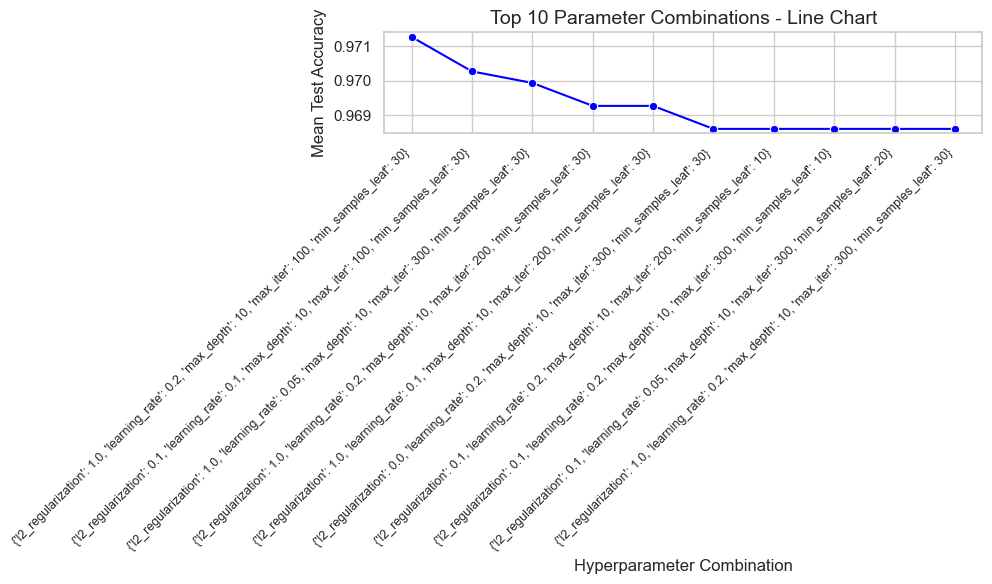
\includegraphics[width=1.1\linewidth]{Graph/hyper parament analysis of histgradient/hyperparameter_combination_line.png}
    \caption{Visual representation of Combination of best fit parameter}
    \label{fig:bestparameter}
\end{figure}
Fig ~\ref{fig:bestparameter} shows the top 10 hyperparameter combinations based on mean test accuracy observed during the grid search. The best-performing configuration achieved a mean test accuracy of approximately 0.9715. Accuracy slightly decreased across the ranked combinations, with the lowest among the top 10 stabilizing at around 0.9692. All top configurations consistently used a \texttt{max\_depth} of 10 and \texttt{min\_samples\_leaf} of 30, suggesting these values contribute significantly to optimal model performance. Variations in \texttt{learning\_rate}, \texttt{l2\_regularization}, and \texttt{max\_iter} had only minor impacts among these top configurations, indicating robustness in the model's accuracy around the best setup.

\begin{figure}[ht]
    \centering
    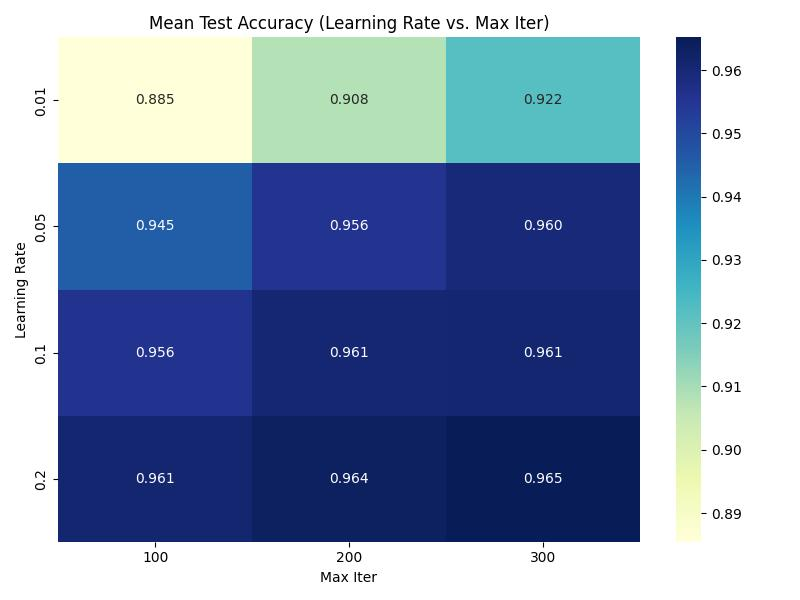
\includegraphics[width=0.9\linewidth]{best_accuracy.jpeg}
    \caption{Achieve higher accuracy based on best-fit combination of learning rate and max iterations.}
    \label{fig:bestaccuracy}
\end{figure}
Fig~\ref{fig:bestaccuracy} presents a heatmap illustrating the impact of varying the \texttt{learning\_rate} and \texttt{max\_iter} on mean test accuracy specifically. Accuracy increases consistently with higher learning rates within the tested range, peaking at a learning rate of 0.2. Additionally, increasing \texttt{max\_iter} generally improves performance, with accuracy stabilizing as \texttt{max\_iter} reaches 300. The best performance (accuracy = 0.965, noted during this specific 2D analysis slice) is achieved at a learning rate of 0.2 with \texttt{max\_iter} set to 300. In contrast, a low learning rate of 0.01 results in significantly poorer accuracy across all iterations, highlighting the importance of this parameter.

\subsection{Evaluation Metrics}\label{sec:evalmetrics}

The performance of each classification model was rigorously evaluated using standard metrics to provide a comprehensive understanding of their predictive capabilities. These metrics were calculated based on the predictions made.

\subsubsection{Confusion Matrix}\label{sec:confmatrix}

The confusion matrix is a fundamental tool used to visualize the performance of a classification algorithm \cite{mahcine}. It provides a breakdown of correct and incorrect predictions for each class. It consists of four key counts:

\begin{itemize}
    \item True Positive (TP): Represents instances where the model correctly predicted the presence of ASD traits.
    \item True Negative (TN): Represents instances where the model correctly predicted the absence of ASD traits.
    \item False Positive (FP): Represents instances where the model incorrectly predicted the presence of ASD traits (Type I error).
    \item False Negative (FN): Represents instances where the model incorrectly predicted the absence of ASD traits when they were actually present (Type II error). This is considered particularly critical in medical diagnostic contexts, as it means a case is missed.
\end{itemize}

\begin{table}[ht]
    \centering
    \caption{Confusion Matrix Metrics of Different Algorithms}
    \label{tab:algorithm_metrics}
    \begin{tabular}{lrrrr}
        \toprule
        \textbf{Algorithm} & \textbf{TN} & \textbf{FP} & \textbf{FN} & \textbf{TP} \\
        \midrule
        Logostic Regression & 274 & 65 & 84 & 326 \\
        Naive Bayes & 306 & 43 & 68 & 332 \\
        Decision Tree (log-loss) & 312 & 27 & 20 & 390 \\
        KNN(Euclidean) & 330 & 19 & 26 & 374 \\
        SVM(RBF) & 334 & 15 & 7 & 393 \\
        Random Forest & 337 & 12 & 18 & 382 \\
        HGBC & 343 & 6 & 10 & 390 \\
        \bottomrule
    \end{tabular}
\end{table}

\subsubsection{Accuracy}\label{sec:accuracy}

Accuracy is defined as the ratio of correctly predicted instances (both true positives and true negatives) to the total number of instances. It provides an overall measure of the model's correctness across both classes. The formula for accuracy is given by:
\begin{equation}
    \text{Accuracy} = \frac{\text{TP} + \text{TN}}{\text{TP} + \text{FP} + \text{TN} + \text{FN}}
    \label{eq:acc}
\end{equation}

\subsection{Precision and Recall Graphical Representation}\label{sec:precision_recall}

The evaluation parameters like precision and recall are mostly useful in evaluating the performance of the trained model. The following has been visually represented by the graphical representation. 

The two factors used to determine the same are listed below:- 

\begin{itemize}
    \item Precision and Recall from Random Forest \hyperref[Fig. 3]{Fig \ref{fig:pre-re-rf}}
    \item Precision and Recall from Support Vector Machine \hyperref[Fig. 4]{Fig \ref{fig:pre-re-svm}}
\end{itemize}

\FloatBarrier

\begin{figure}[H]
    \centering
    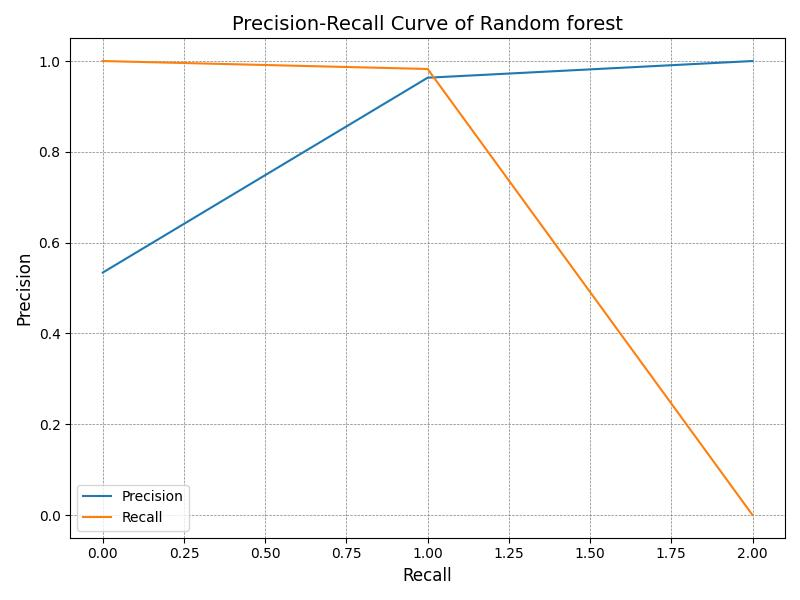
\includegraphics[width=0.8\linewidth]{Graph/precision and recall graph/pre_re_rf.jpeg}
    \caption{Precision and Recall Graph: Random Forest}
    \label{fig:pre-re-rf}
\end{figure}

\begin{figure}[h]
    \centering
    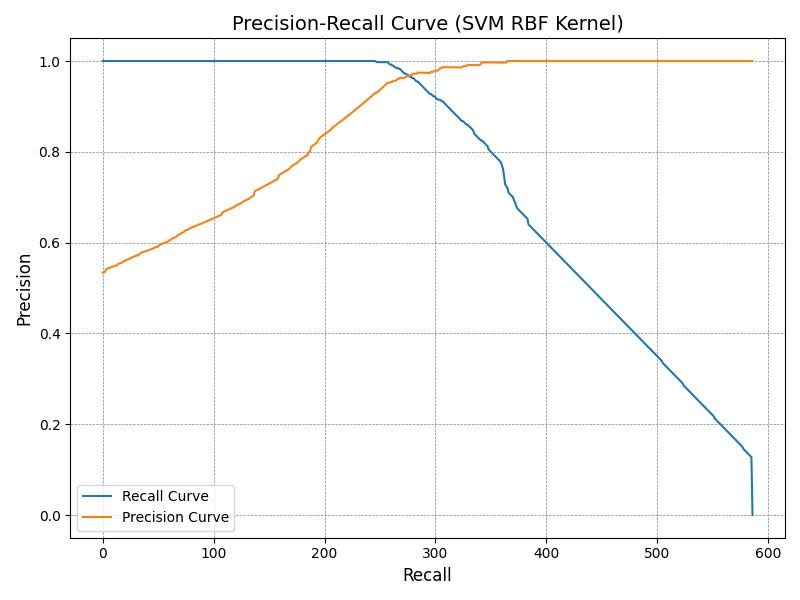
\includegraphics[width=0.8\linewidth]{Graph/precision and recall graph/pre_re_svm.jpeg}
    \caption{Precision and Recall Graph: Support Vector Machine (SVF)}
    \label{fig:pre-re-svm}
\end{figure}


\subsection{F1 Score}\label{sec:f1score}

The F1 Score is the harmonic mean of precision and recall. It is calculated to balance the trade-off between these two metrics and is particularly useful when dealing with imbalanced datasets, where high precision or recall alone might not reflect overall performance well \cite{mahcine}. A high F1 score indicates a good balance between precision and recall. The formula for the F1 Score is:
\begin{equation}
    \text{F1 Score} = 2 \cdot \frac{\text{Precision} \cdot \text{Recall}}{\text{Precision} + \text{Recall}}
    \label{eq:f1}
\end{equation}

\subsection{Result Analysis}\label{sec:results}

The performance of the different supervised machine learning models on the ASD prediction task was analyzed based on the evaluation metrics calculated from the test set predictions. The results highlight the varying effectiveness of the models for this specific dataset, as presented for all models in \hyperref[tab:algorithm_metrics]{Table~\ref{tab:algorithm_metrics}} and \hyperref[tab:Performance_Matrix]{Table~\ref{tab:Performance_Matrix}}.

\begin{table*}[ht]
    \centering
    \caption{Performance Matrix Including All Parameters}
     \renewcommand{\arraystretch}{1.5} % Taller rows
      \setlength{\tabcolsep}{1pt} % Wider columns
    \begin{tabular}{|c|l|c|c|c|c|}
        \hline
        \textbf{No.} & \textbf{Algorithms} & \textbf{Accuracy(\%)} & \textbf{Precision(\%)} & \textbf{Recall(\%)} & \textbf{F1-Score(\%)} \\
        \hline
          1  & Logistic Regression & 80.11 & 83.38 & 79.51 & 81.40 \\
          \hline
          2 & Naive Bayes & 85.18 & 88.53 & 83.00 & 85.68 \\
          \hline
          3 & Decision Tree & 93.72 & 93.53 & 95.12 & 94.32 \\
          \hline
          4 & k-nearest neighbor & 93.99 & 95.17 & 94.30 & 94.33 \\
          \hline
          5 & Support Vector Machine & 97.06 & 96.32 & 98.25 & 97.28 \\
          \hline
          6 & Random Forest & 95.99 & 96.95 & 95.50 & 96.22 \\
          \hline
          7 & HGBC & 97.86 & 98.48 & 97.50 & 97.90 \\
          \hline
    \end{tabular}
    \label{tab:Performance_Matrix}
\end{table*}


The overall accuracy achieved by each model is compared and visualized in \hyperref[fig:acc]{Fig~\ref{fig:acc}}.

\begin{figure}[ht]
    \centering
    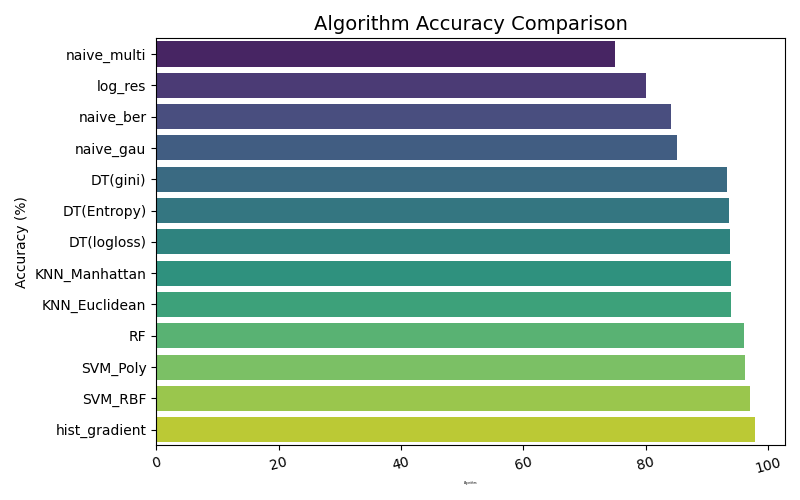
\includegraphics[width=1\linewidth]{accuracy.png}
    \caption{Accuracy of the different classification techniques}
    \label{fig:acc}
\end{figure}

It can be observed from \hyperref[tab:Performance_Matrix]{Table~\ref{tab:Performance_Matrix}} and \hyperref[fig:acc]{Fig~\ref{fig:acc}} that the HGBC attained the highest accuracy of 97.86\%, significantly outperforming simpler models like Logistic Regression (80.11\%) and Naive Bayes (85.18\%). The SVM with an RBF kernel also demonstrated strong performance, achieving 97.06\% accuracy, closely following HGBC. Other models like Random Forest (95.99\%), KNN (93.99\%), and Decision Tree (93.72\%) also showed respectable accuracy levels, indicating their general suitability for this type of classification problem.

Visual representations of precision and recall for the top-performing models are also provided in \hyperref[fig:pre-re-hist]{Fig~\ref{fig:pre-re-hist}}, \hyperref[fig:pre-re-svm]{Fig~\ref{fig:pre-re-svm}}, and \hyperref[fig:pre-re-rf]{Fig~\ref{fig:pre-re-rf}}. HGBC again shows leading performance with high precision (98.48\%) and recall (97.50\%), indicating a strong ability to both correctly identify positive cases (high recall) and minimize incorrect positive predictions (high precision). SVM also performs remarkably well in this regard, particularly achieving a very high recall (98.25\%), meaning it is highly effective at identifying individuals with ASD traits, though its precision is slightly lower than HGBC (96.32\%). Random Forest shows a good balance between precision (96.95\%) and recall (95.50\%). The choice between HGBC and SVM might depend on whether minimizing False Positives (favoring HGBC's higher precision) or minimizing False Negatives (favoring SVM's slightly higher recall) is deemed more critical for the application.


The F1 Score (defined in \hyperref[sec:f1score]{Section~\ref{sec:f1score}}) provides a single metric that balances precision and recall, which is particularly useful when dealing with imbalanced datasets, where high precision or recall alone might not reflect overall performance well. The F1 Scores for all models are visualized in \hyperref[fig:f1_score]{Fig~\ref{fig:f1_score}}.

\begin{figure}[ht]
    \centering
    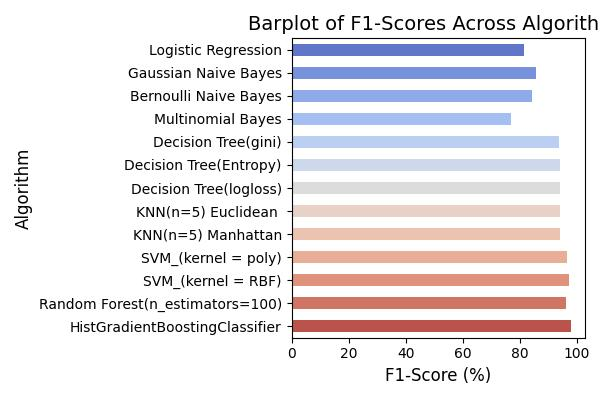
\includegraphics[width=0.8\linewidth]{Graph/DS/f1_score.jpeg}
    \caption{Visual Representation of comparing all the classification model based on F1-score}
    \label{fig:f1_score}
\end{figure}

As shown in \hyperref[fig:f1_score]{Fig~\ref{fig:f1_score}}, the HGBC model achieves the highest F1 Score (which would be approximately 97.99\% based on the calculated precision and recall), closely followed by SVM (approximately 97.28\%). This further reinforces the finding that HGBC is the most effective model among those tested for this classification task, offering the best overall balance between correctly identifying positive cases and limiting false positives. The performance across models, as measured by the F1 score, largely mirrors the trend observed with accuracy.

The analysis of hyperparameter tuning for HGBC (\hyperref[fig:bestparameter]{Fig~\ref{fig:bestparameter}} and \hyperref[fig:bestaccuracy]{Fig~\ref{fig:bestaccuracy}}) indicates that the model's performance is sensitive to parameters like learning rate and maximum iterations, with optimal accuracy being achieved within specific ranges. A learning rate of 0.2 and maximum iterations of 300, combined with a max depth of 10 and min samples leaf of 30, were found to contribute to the highest accuracy during the tuning process. The high performance of the tuned HGBC model on the evaluation metrics supports its selection as the best predictive model for this dataset.

Overall, the results indicate that ensemble methods, particularly Histogram Gradient Boosting and Random Forest, along with Support Vector Machines, are well-suited for predicting ASD traits based on the provided dataset, with the hyperparameter-tuned HGBC demonstrating superior performance across key metrics including accuracy, precision, recall, and F1-score.


\subsection{Exploratory Data Analysis}
\label{sec:data_analysis}

\subsubsection{\textbf{Distribution Based on Ethnicity}}

Exploratory data analysis has been applied on this dataset and it is explored that ASD traits are more prevalent in White Europeans. It is based on various factors. There are various potential explanations that could be genetic, social, environmental and many more. Although, environmental factors can vary on various ethnic clusters and geographic regions.

\textbf{Diet and lifestyle} can also play a vital role to develop neuro-developmental conditions.

\textbf{Awareness} about the ASD plays another major factor. White Europeans are more aware than other ethnic clusters as visualized in \hyperref[fig:ethni]{Fig \ref{fig:ethni}}. They can access specialized testing for ASD. That is the reason for higher diagnostic rate in white Europeans as compared to other ethnicity where awareness might be lower or they may not prioritize the ASD identifications.

Distribution based on Ethnicity:

\begin{figure}[ht]
    \centering
    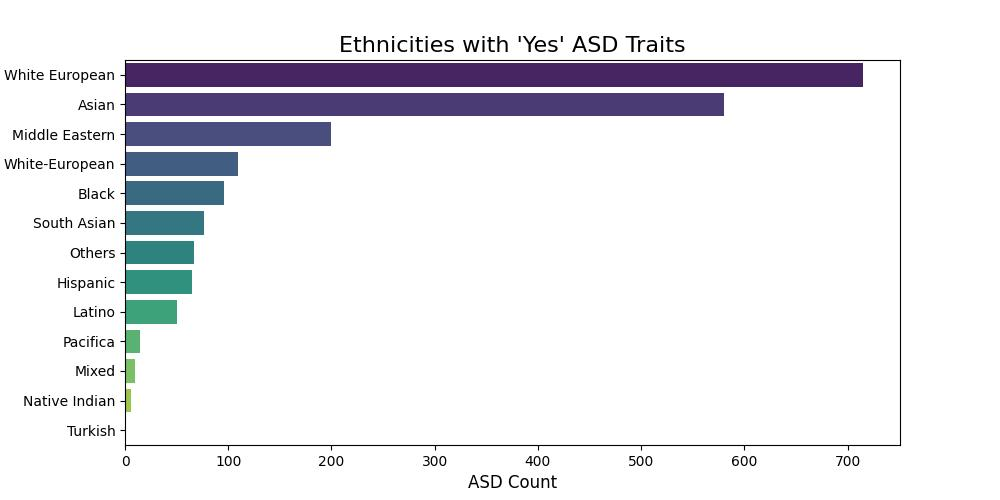
\includegraphics[width=1\linewidth]{Graph/EDA/Ethnicity_yes.jpeg}
    \caption{The ethnics with the ASD traits as \enquote{YES}}
    \label{fig:ethni}
\end{figure}

\subsubsection{Distribution Based on Sex:}
The observation has shown that males tend to exhibit more ASD traits compared to females as visualized in \hyperref[fig:gen]{Fig \ref{fig:gen}}. One potential contributing factor is hormonal differences, particularly the role of testosterone in brain development and its possible link to ASD. Research suggests that prenatal exposure to higher levels of testosterone may increase the likelihood of developing ASD-related traits. Since females generally have lower levels of testosterone than males, this hormonal disparity could partly explain the higher prevalence of ASD traits in males.

\begin{figure}[ht]
    \centering
    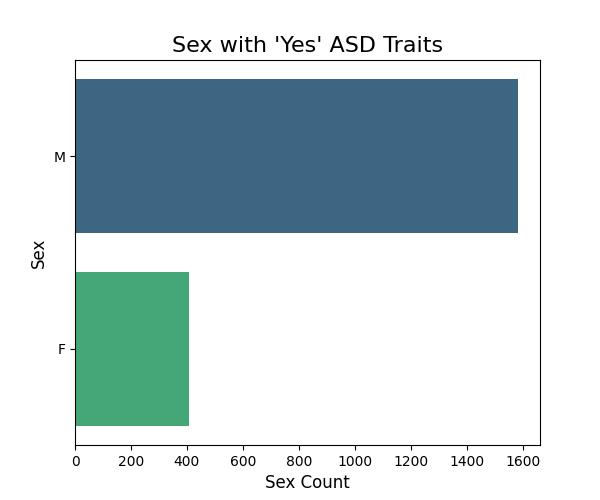
\includegraphics[width=0.8\linewidth]{Graph/EDA/sex.jpeg}
    \caption{Gender distribution with ASD traits as \enquote{YES}}
    \label{fig:gen}
\end{figure}


\subsubsection{Distribution Based on Age Category}

Thus we have found that ASD has more potential towards affective children between the age of 2-12 years as visualized in \hyperref[fig:age]{Fig \ref{fig:age}} and in \hyperref[tab:age-category]{Table~\ref{tab:age-category}}.

Distribution based on Age Category:
\begin{figure}[ht]
    \centering
    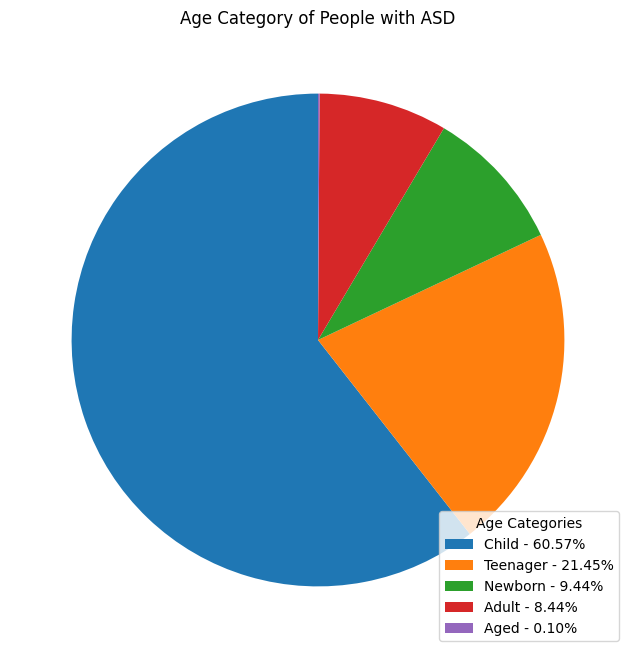
\includegraphics[width=0.8\linewidth]{Graph/EDA/age_chart.png}
    \caption{Age categories distribution of ASD traits:}
    \label{fig:age}
\end{figure}

\begin{table}[ht]
    \centering
    \caption{Age Category Traits in Percentage}
    \vspace{0.8em}
    \renewcommand{\arraystretch}{1.5} % Taller rows
    \setlength{\tabcolsep}{20pt}     % Wider columns
    \begin{tabular}{|c|c|}
        \hline
        \textbf{Age Category} & \textbf{Traits (\%)} \\
        \hline
        Newborn & 9.44\% \\
        \hline
        Child & 60.57\% \\
        \hline
        Teenager & 21.45\% \\
        \hline
        Adult & 8.44\% \\
        \hline
        Aged & 0.10\% \\
        \hline
    \end{tabular}
    \label{tab:age-category}

    \small
    \noindent

\end{table}

\subsubsection{Distribution Based on Genetics} Based on the analysis of the dataset, it appears that most individuals’ family members do not have ASD traits, nor do they possess ASD traits themselves. This suggests that genetic factors may not play a dominant role in the prevalence of ASD traits as visualized in \hyperref[fig:genetics]{Fig \ref{fig:genetics}}. Instead, environmental influences—such as parental neglect, inappropriate behavior, or lack of socialization—may contribute more significantly to the development of these traits.

\begin{figure}[!ht]
    \centering
    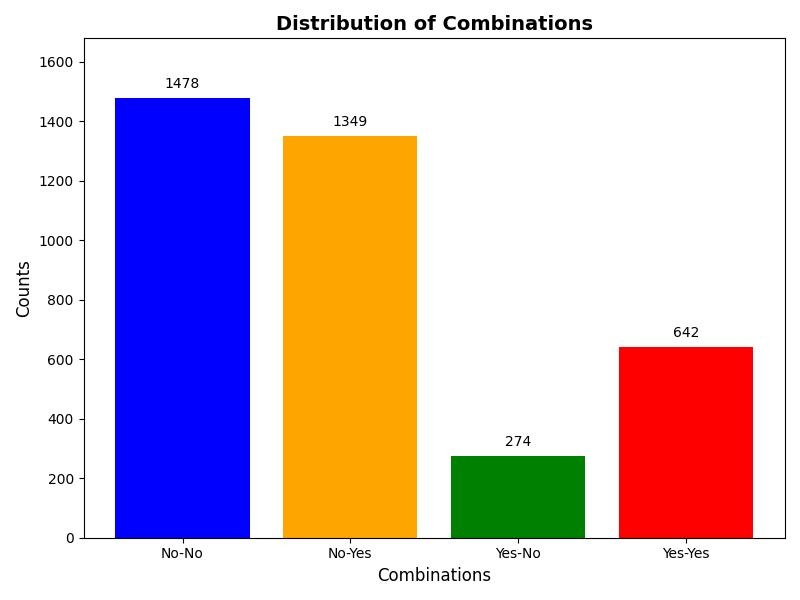
\includegraphics[width=0.8\linewidth]{Graph/EDA/fam_mem.jpeg}
    \caption{confusion matrix styled labeled graphical representation of the distribution of family member traits of ASD}
    \label{fig:genetics}
\end{figure}

\section{Conclusion}
\label{sec:conclusion}
The potential of machine learning to enhance clinical evaluations for Autism Spectrum Disorder (ASD) is demonstrated by this work. The study investigated the effectiveness of several supervised machine learning classification algorithms, including Logistic Regression, Decision Trees, KNN, Naive Bayes, Random Forest, SVM, and HGBC, in predicting the presence of ASD traits based on a quantitative dataset.

A primary finding was the identification of the most effective model. The HGBC achieved the highest predictive performance among the evaluated algorithms. An accuracy of 97.86\% was attained by the HGBC model, significantly outperforming simpler models like Logistic Regression (80.11\%) and Naive Bayes (85.18\%). The superior performance of HGBC was further corroborated by high precision (98.48\%), recall (97.50\%), and an F1 Score (97.90\%), indicating a strong ability to both correctly identify positive cases and minimize false alarms. Strong performance was also observed with the SVM (RBF kernel) and Random Forest models, achieving accuracies of 97.06\% and 95.99\%, respectively.

The exploratory data analysis provided crucial insights into the characteristics of the dataset and the distribution of ASD traits. Notably, analysis of the age distribution revealed that ASD traits were most prevalent among children, affecting 60.57\% of individuals in this age category within the dataset, indicating a significant susceptibility during younger years. Furthermore, the dataset indicated that ASD traits were observed more frequently in males compared to females. Patterns related to ethnicity (higher prevalence noted in White Europeans) and family history (genetic factors appearing less dominant in this specific dataset) were also identified, suggesting the complex interplay of multiple factors.

These findings highlight the potential of machine learning models, particularly HGBC, as valuable tools that could complement traditional clinical assessments for early ASD detection. Earlier interventions, consistently shown to improve outcomes for individuals with ASD, could be facilitated by more accurate and timely screening.

Further advancements in prediction performance are anticipated as machine learning techniques continue to develop and more comprehensive datasets become available. The integration of these technologies into clinical practice is expected to transform ASD screening programs by offering scalable and efficient methods. Consequently, a critical step in applying computational methods to address a significant public health challenge is marked by the results presented in this paper.

\begin{thebibliography}{99}
\bibitem{1in31}
Centers for Disease Control and Prevention (2024) Autism Spectrum Disorder (ASD) - Data and Statistics. Accessed: 2025-04-20.

\bibitem{ini3}
Lord, C., Rutter, M. and Le Couteur, A. (1994) Autism Diagnostic Interview-Revised: A revised version of a diagnostic interview for caregivers of individuals with possible pervasive developmental disorders. \emph{Journal of Autism and Developmental Disorders} \textbf{24}(5), 659--685. doi:10.1007/BF02172145

\bibitem{bib12}
Stevens, E., Dixon, D. R., Novack, M. N., Granpeesheh, D., Smith, T. and Linstead, E. (2019) Identification and analysis of behavioral phenotypes in autism spectrum disorder via unsupervised machine learning. \emph{International Journal of Medical Informatics} \textbf{129}, 29--36. doi:10.1016/j.ijmedinf.2019.05.006

\bibitem{bib14}
Prasad, V., Sriramakrishnan, G.V. and Diana Jeba Jingle, I. (2023) Autism spectrum disorder detection using brain MRI image enabled deep learning with hybrid sewing training optimization. \emph{Signal, Image and Video Processing} \textbf{17}, 4001--4008. doi:10.1007/s11760-023-02630-y

\bibitem{parlett2023applications}
Parlett-Pelleriti, C. M., Stevens, E., Dixon, D. et al. (2023) Applications of Unsupervised Machine Learning in Autism Spectrum Disorder Research: a Review. \emph{Review Journal of Autism and Developmental Disorders} \textbf{10}, 406--421. doi:10.1007/s40489-021-00299-y

\bibitem{nogay2020machine}
Nogay, H. S. and Adeli, H. (2020) Machine learning (ML) for the diagnosis of autism spectrum disorder (ASD) using brain imaging. \emph{Reviews in the Neurosciences} \textbf{31}(8), 825--841. doi:10.1515/revneuro-2020-0043

%\bibitem{bib3}
%Parlett-Pelleriti, C. M., Stevens, E., Dixon, D. et al. (2023) Applications of Unsupervised Machine Learning in Autism Spectrum Disorder Research: a Review. \emph{Review Journal of Autism and Developmental Disorders} \textbf{10}, 406--421. doi:10.1007/s40489-021-00299-y

\bibitem{bib4}
Vakadkar, K., Purkayastha, D. and Krishnan, D. (2021) Detection of Autism Spectrum Disorder in Children Using Machine Learning Techniques. \emph{SN Computer Science} \textbf{2}, 386. doi:10.1007/s42979-021-00776-5

\bibitem{bib5}
Alves, C. L., Toutain, T. G. L. d. O., de Carvalho Aguiar, P. et al. (2023) Diagnosis of Autism Spectrum Disorder Based on Functional Brain Networks and Machine Learning. \emph{Scientific Reports} \textbf{13}, 8072. doi:10.1038/s41598-023-34650-6

\bibitem{bib6}
Mellema, C. J., Nguyen, K. P., Treacher, A. et al. (2022) Reproducible Neuroimaging Features for Diagnosis of Autism Spectrum Disorder with Machine Learning. \emph{Scientific Reports} \textbf{12}, 3057. doi:10.1038/s41598-022-06459-2

\bibitem{bib7}
Zhou, Y., Jia, G., Ren, Y. et al. (2024) Advancing ASD Identification with Neuroimaging: A Novel GARL Methodology Integrating Deep Q-Learning and Generative Adversarial Networks. \emph{BMC Medical Imaging} \textbf{24}, 186. doi:10.1186/s12880-024-01360-y

\bibitem{bib8}
Rajagopalan, S. S., Zhang, Y. and Yahia, A. (2024) [Title not provided -- please update with article title]. \emph{JAMA Network Open} \textbf{7}(8), e2429229. doi:10.1001/jamanetworkopen.2024.29229

\bibitem{bib10}
Jaradat, A. S., Wedyan, M., Alomari, S. and Barhoush, M. M. (2025) Using Machine Learning to Diagnose Autism Based on Eye Tracking Technology. \emph{Diagnostics} \textbf{15}(1), 66. doi:10.3390/diagnostics15010066

\bibitem{bib13}
Eslami, T. and Saeed, F. (2021) Explainable and scalable machine learning algorithms for detection of autism spectrum disorder using fMRI data. In El-Baz, A. S. and Suri, J. S. (eds.) \emph{Neural Engineering Techniques for Autism Spectrum Disorder}, pages 39-54. Academic Press. doi:10.1016/B978-0-12-822822-7.00004-1

\bibitem{datapre}
Kotsiantis, S., Kanellopoulos, D. and Pintelas, P. (2006) Data Preprocessing for Supervised Learning. \emph{International Journal of Computer Science} \textbf{1}, 111--117.

\bibitem{hosmer2000applied}
Hosmer, D. W. and Lemeshow, S. (2000) \emph{Applied Logistic Regression}. 2nd edition. Wiley, New York.

\bibitem{decision}
Mienye, I. D. and Jere, N. (2024) A Survey of Decision Trees: Concepts, Algorithms, and Applications. \emph{IEEE Access} \textbf{12}, 86716--86727. doi:10.1109/ACCESS.2024.3416838

\bibitem{KNN}
Taunk, K., De, S., Verma, S. and Swetapadma, A. (2019) A Brief Review of Nearest Neighbor Algorithm for Learning and Classification. In \emph{2019 International Conference on Intelligent Computing and Control Systems (ICCS)}, pages 1255-1260. doi:10.1109/ICCS45141.2019.9065747

\bibitem{naive}
Chen, H., Hu, S., Hua, R. et al. (2021) Improved naive Bayes classification algorithm for traffic risk management. \emph{EURASIP J. Adv. Signal Process} \textbf{2021}(30).

\bibitem{rand}
Breiman, L. (2001) Random Forests. \emph{Machine Learning} \textbf{45}(1), 5--32. doi:10.1023/A:1010933404324

\bibitem{svm}
Hearst, M. A., Dumais, S. T., Osuna, E., Platt, J. and Scholkopf, B. (1998) Support vector machines. \emph{IEEE Intelligent Systems and their Applications} \textbf{13}(4), 18--28. doi:10.1109/5254.708428

\bibitem{hist}
Maftoun, M., Shadkam, N., Komamardakhi, S. S. S., Mansor, Z. and Joloudari, J. H. (2024) Malicious URL Detection using optimized Hist Gradient Boosting Classifier based on grid search method. arXiv preprint arXiv:2404.13050.

\bibitem{para}
Ilemobayo, J., Durodola, O., Alade, O., Awotunde, O., Adewumi, T., Falana, O., Ogungbire, A., Osinuga, A., Ogunbiyi, D., Odezuligbo, I., Edu, O. and Ifeanyi, A. (2024) Hyperparameter Tuning in Machine Learning: A Comprehensive Review. \emph{Journal of Engineering Research and Reports} \textbf{26}, 388--395. doi:10.9734/jerr/2024/v26i61188

\bibitem{mahcine}
Bishop, C. M. (2006) \emph{Pattern Recognition and Machine Learning}. Springer, New York, NY.


\end{thebibliography}
\end{document}